\begin{filecontents}{\jobname.bib}
    %[1] (\cite{jo2021})
    @article{jo2021,
        author = {Jo,J. and Chae,Y. and Jang,H. and Kong,J.},
        title = {Federated-Access Management System and Videoconferencing Applications: Results from a Pilot Service during COVID-19 Pandemic},
        journal = {Multidisciplinary Digital Publishing Institute (MDPI)},
        pages = {1--19},
        year = {2021},
        volume = {Electronics 2021,10, 2239},
        DOI = {https://doi.org/10.3390/electronics10182239},
        url = {https://www.researchgate.net/publication/354545424_Federated-Access_Management_System_and_Videoconferencing_Applications_Results_from_a_Pilot_Service_during_COVID-19_Pandemic}
    }
    %[2] (\cite{bispham2021})
    @article{bispham2021,
        author = {Bispham,M.K. and Creese,S. and Dutton,W.H. and Esteve-Gonzalez,P. and Goldsmith,M.},
        title = {Cybersecurity in Working from Home: An Exploratory Study},
        journal = {SSRN Electronic Journal},
        pages = {1--43},
        year = {2021},
        volume = {January 2021},
        DOI = {https://doi.org/10.2139/ssrn.3897380},
        url = {https://www.researchgate.net/publication/353661008_Cybersecurity_in_Working_from_Home_An_Exploratory_Study}
    }
    %[3] (\cite{ozer2024})
    @article{ozer2024,
        author = {Ozer,M. and Kose,Y. and Kucukkaya,G. and Varlioglu,E.R.},
        title = {The Shifting Landscape of Cybersecurity: The Impact of Remote Work and COVID-19 on Data Breach Trends},
        journal = {IEEE Computer Science and Computer Engineering (CSCE)},
        year = {2024},
        url = {https://arxiv.org/html/2402.06650v2}
    }
    %[4] (\cite{salloum2021})
    @article{salloum2021,
        author = {Salloum,S. and Gaber,T. and Vadera,S. and Shaalan,K.},
        title = {Phishing Email Detection Using Natural Language Processing Techniques: A Literature Survey},
        journal = {Procedia Computer Science},
        pages = {19--28},
        year = {2021},
        volume = {189},
        DOI = {https://doi.org/10.1016/j.procs.2021.05.077},
        url = {https://www.sciencedirect.com/science/article/pii/S1877050921011741}
    }
    %[5] (\cite{jennings2021})
    @article{jennings2021,
        author = {Jennings,R.},
        title = {Zoom #fails grow: 530,000 passwords leaked, details for sale by hacker},
        journal = {TechBeacon},
        year = {2021},
        url = {https://techbeacon.com/security/zoom-fails-grow-530000-passwords-leaked-details-sale-hacker}
    }
    %[6] (\cite{condeco2024})
    @article{condeco2024,
        title = {How to Decide Who Should Attend Your Meeting?},
        journal = {Condeco},
        year = {2024},
        url = {https://www.cnbc.com/2021/08/01/zoom-reaches-85-million-settlement-over-user-privacy-and-hacker-zoombombing.html}
    }
    %[7] (\cite{golkarnarenji2012})
    @article{golkarnarenji2012,
        author = {Golkarnarenji,G. and Ali,U.},
        title = {Unified Communications Security : A study of IT personnel awareness on video conferencing security recommendations},
        journal = {Department of Computer science, Electrical and Space Engineering, Lulea University of Technology},
        pages = {1--114},
        year = {2012},
        url = {https://www.academia.edu/3056220/Unified_Communications_Security_A_study_of_IT_personnel_awareness_on_video_conferencing_security_recommendations}
    }
    %[8] (\cite{culafi2023})
    @article{culafi2023,
        author = {Culafi,A.},
        title = {Microsoft AI researchers mistakenly expose 38 TB of data},
        journal = {TechTarget},
        year = {2023},
        url = {https://www.techtarget.com/searchsecurity/news/366552399/Microsoft-AI-researchers-mistakenly-expose-38-TB-of-data}
    }
    %[9] (\cite{kumar2017})
    @article{kumar2017,
        author = {Kumar,S. and Mahajan,R. and Kumar,N. and Khatri,S.K.},
        title = {A study on web application security and detecting security vulnerabilities},
        journal = {IEEE},
        pages = {451-455},
        year = {2017},
        volume = {09},
        DOI = {https://doi.org/10.1109/ICRITO.2017.8342469},
        url = {https://ieeexplore.ieee.org/document/8342469}
    }
    %[10] (\cite{karl2021})
    @article{karl2021,
        author = {Karl,K.A. and Peluchette,J.V. and Aghakhani,N.},
        title = {Virtual Work Meetings During the COVID-19 Pandemic: The Good, Bad, and Ugly},
        journal = {Sage},
        pages = {343-365},
        year = {2021},
        volume = {53(3)},
        DOI = {https://doi.org/10.1177/10464964211015286},
        url = {https://journals.sagepub.com/doi/full/10.1177/10464964211015286}
    }
    %[11] (\cite{hasan2021})
    @article{hasan2021,
        author = {Hasan,R. and Hasan,R.},
        title = {Towards a Threat Model and Security Analysis of Video Conferencing Systems},
        journal = {IEEE Consumer Communications and Networking Conference (CCNC)},
        pages = {1-4},
        year = {2021},
        volume = {01},
        DOI = {https://doi.org/10.1109/CCNC49032.2021.9369505},
        url = {https://www.researchgate.net/publication/349994212_Towards_a_Threat_Model_and_Security_Analysis_of_Video_Conferencing_Systems}
    }
    %[12] (\cite{isobe2021})
    @article{isobe2021,
        author = {Isobe,T. and Ito,R.},
        title = {Security Analysis of End-to-End Encryption for Zoom Meetings},
        journal = {IEEE Access},
        pages = {90677-90689},
        year = {2021},
        volume = {09},
        DOI = {https://doi.org/10.1109/ACCESS.2021.3091722},
        url = {https://ieeexplore.ieee.org/document/9462825?denied=}
    }
    %[13] (\cite{arishina2022})
    @article{arishina2022,
        author = {Arishina,Y. and Hu,Y.F. and Hoppa,M.A.},
        title = {A Study of Video ConferencingSoftware Risks and Mitigation Strategies},
        journal = {Journal of The Colloquium for Information Systems Security Education},
        pages = {1-10},
        year = {2022},
        volume = {09},
        DOI = {https://doi.org/10.53735/cisse.v9i1.134},
        url = {https://cisse.info/journal/index.php/cisse/article/view/134/134}
    }
    %[14] (\cite{tondel2022})
    @article{tondel2022,
        author = {Tondel,I.A. and Cruzes,D.S.},
        title = {Continuous software security through security prioritisation meetings},
        journal = {Elsevier},
        pages = {1-25},
        year = {2022},
        volume = {194},
        DOI = {https://doi.org/10.1016/j.jss.2022.111477},
        url = {https://www.sciencedirect.com/science/article/pii/S0164121222001625}
    }
\end{filecontents}
\documentclass[a4paper, 12pt]{article}
\usepackage[left=1in,right=1in,top=1in,bottom=1in]{geometry}
\usepackage{setspace}
\usepackage{titlesec}
\usepackage{graphicx}
\usepackage[section]{placeins}
\usepackage[bookmarks]{hyperref}
\usepackage[super]{nth}
\usepackage{subfig}
\usepackage{makeidx}
\usepackage{hyperref}
\usepackage{acronym}
\usepackage{array} 
\usepackage[backend=biber,style=authoryear,autocite=inline, maxbibnames=9 ]{biblatex}
\DeclareNameAlias{sortname}{last-first}
\addbibresource{\jobname.bib}
\graphicspath{ {images/} }
\newcolumntype{C}{>{$\displaystyle}l<{$}}

\makeindex

\begin{document}
    % 01 - Title page
    \newpage
    \pagenumbering{none}
    \begin{figure}
        \centering
        \vspace*{0cm}
\includegraphics[width=0.35\textwidth]{uoc_logo.jpg}
    \end{figure}
    \begin{center}
        \begin{LARGE}  
            \textbf{Information Security and Risk\\ Assessment associated with}
            \textbf{meeting modes}
        \end{LARGE}  
        \break\break
        By\\
        \textbf{M.M.A.S.T. Akmeemana - Index No: 20020015\\ A.I. Vidanage - Index No: 20021089\\ K.P.G.K. Jayathilake - Index No: 20020521}
        \break\break
        \textbf{Supervisor: Dr. C.I. Kappetiyagama\\ Co-supervisor: Mr. Tharindu Wijethilaka}
        \break\break
        \begin{large}  
            IS 4101 – Final Year Project in Informatioon Systems
            \break\break
            Degree of Bachelor of Science Honours in\\ Information Systems
            \break\break
        \end{large}
        
        \begin{figure}[h]
            \centering
            
\includegraphics[width=0.3\textwidth]{ucsc_logo.png}
        \end{figure}
        \begin{large}  
            University of Colombo School of Computing\\
            35, Reid Avenue, Colombo 07,\\
            Sri Lanka\\
            April 2024
        \end{large}
    \end{center}

    % 02 - Table of Contents page
    \newpage
    \addcontentsline{toc}{section}{Table of Contents}
    \section*{\begin{LARGE} Table of Contents \end{LARGE} }
    \pdfbookmark{\contentsname}{toc}
    \tableofcontents

    \begin{spacing}{1.0}
    % 03 - Introduction page
    \newpage
    \pagenumbering{arabic}
    \section{Introduction} 
    \indent \par Meetings are vital for any organization as they enable collaboration, decision-making, and the exchange of crucial information. However, to ensure their success, meetings must be carefully planned and organized. This involves addressing key questions: Do we truly need to hold a meeting? Who should be invited? And what is the best format for the meeting --- online, onsite, or hybrid ?
    \newline\newline \textbf{The Changing Landscape of Meetings}: Before the COVID-19 pandemic, discussions about meeting security and privacy were less prevalent, as most meetings were conducted onsite with the physical presence of attendees. The pandemic has significantly altered this landscape, expanding meeting modes to include online and hybrid formats, in addition to traditional onsite meetings. Since 2020, the usage of online meeting platforms has surged due to quarantine restrictions and the need for remote collaboration (\cite{jo2021}).
    \newline\newline \textbf{Security and Privacy Concerns}: The shift towards online and hybrid meetings has brought security and privacy issues to the forefront. In the Information Technology sector, many participants possess a sound understanding of information security (\cite{golkarnarenji2012}). However, even knowledgeable individuals can make errors, especially as the complexity of the scenarios increases (\cite{culafi2023}). Human decision-making is often influenced by emotions and biases, which can lead to mistakes. This is equally applicable in the context of organizing meetings, where improper use of online platforms can result in financial, reputational,and losses of proprietary information, capital and corporate value.
    \newline\newline \textbf{Selecting the Right Participants}: One of the most critical aspects of organizing a meeting is inviting the right participants. Although this may seem straightforward, it is often a rushed or overlooked step. The success and productivity of a meeting largely depend on having the appropriate individuals present, whether in person or virtually. Selecting the right attendees is crucial because their background and capabilities can influence the meeting's mode and effectiveness. Moreover, having the right participants is essential for maintaining the confidentiality of the information shared during the meeting. When only the necessary and relevant individuals are present, the risk of information leakage is minimized, and sensitive discussions can be conducted securely. Cognitive and organizational bias undermines good decision-making.
    \par To ensure a successful and secure meeting, consider the following principles for selecting participants:
    \begin{enumerate}
        \item \textbf{Need}: Identify who is essential based on their relevance to the meeting's topic and their ability to contribute significantly to the discussions. These are the individuals whose presence is crucial for the meeting's success and whose involvement ensures that confidentiality is preserved.
        \item \textbf{Want}: Differentiate between those whose presence is desired but not critical. While these individuals might add value, they are not essential unless they can provide meaningful contributions to the meeting's agenda and help maintain the meeting's confidentiality.
        \item \textbf{Value}: Assess the potential value each attendee brings. The goal is to ensure that all participants can contribute to achieving the desired outcomes, whether that involves making decisions, offering insights, or advancing solutions. Their involvement should also align with the need to safeguard the information discussed.
    \end{enumerate}
    \par By carefully selecting participants based on need, want, and value, you align the attendees with the meeting’s goals, ensuring that each meeting is productive and purposeful. Clear objectives will guide you in choosing the right people, leading to more effective and efficient meetings. Moreover, this thoughtful selection process enhances the confidentiality of the information shared, ensuring that sensitive topics remain secure and are only accessible to those who are truly relevant.
    \par Accordingly, during our research project, we will explore whether it is possible to identify a relationship among security and privacy-related factors of a meeting including participants, capabilities of participants, documents, and data shared in the meeting and meeting mode. After identifying such a relationship, we expect to evaluate conformance of the relationship with real world scenarios accurately. Then future researchers will be able to use our findings with confidence, to proceed further in our research path associated with meeting security and privacy.

    % 04 - Background, theory, related work, research gap and statement of the problem
    \section{Background, theory, related work, research gap and statement of the problem}

    \subsection{Background}
    \indent \par Meetings are an integral part of organizational operations, serving as platforms for collaboration, decision-making, and the exchange of essential information. Traditionally, most meetings were conducted onsite, with participants physically present in a designated location. However, the COVID-19 pandemic has transformed the landscape of how meetings are held, leading to a significant rise in online and hybrid meeting formats. This shift has brought new challenges and considerations, particularly concerning the security and confidentiality of information shared during meetings.
    \par Prior to the pandemic, meetings were mainly held in person, and security concerns were largely physical --- ensuring that meeting rooms were secure and that unauthorized persons were not present. The rapid adoption of online meeting platforms since 2020 has necessitated a reevaluation of these security paradigms (\cite{jo2021}). The "new normal" of remote work has highlighted the vulnerabilities inherent in digital communications, with security breaches and privacy issues becoming more frequent and complex (\cite{bispham2021})(\cite{ozer2024}).
    \par The increase in remote work and the reliance on online meeting platforms have led to a spike in reported security incidents (\cite{jo2021})(\cite{bispham2021}). These platforms, while convenient, have been found to have various security flaws, ranging from phishing attacks to unauthorized access and data breaches (\cite{ozer2024}). Early in the pandemic, many popular meeting platforms faced inspection over their inadequate security measures, which were quickly exploited as their usage increased (\cite{jennings2021}). Although improvements have been made, the challenge of securing online meetings remains prominent. However, irrespective of the meeting mode, any opportunities given to the wrong attendees for the meeting can give room for the insecurity of the meeting and the attack surface can be increased. 
    \par Research into the security issues associated with the "Work From Home" culture has shown a marked increase in vulnerabilities, particularly in digital communication tools. Studies indicate that phishing and other cyberattacks have targeted the expanded digital workspace, exploiting both technological and human weaknesses (\cite{salloum2021}). Furthermore, while the security of online meetings has received significant attention, there is a noticeable lack of comprehensive strategies addressing the secure organization and execution of meetings based on the sensitivity of the information discussed and the selection of participants.
    \par A critical aspect of meeting organization is the selection of participants. Ensuring that the right people are invited to a meeting is not only a matter of operational efficiency but also of maintaining the confidentiality and security of the information shared. Inappropriate or unnecessary attendees can increase the risk of information leakage and compromise the meeting's objectives. Therefore, a systematic approach to selecting participants, based on their relevance and the nature of the information being discussed, is essential for maintaining security (\cite{condeco2024}).

    \subsection{Theory}
    \indent \par For now, based on our literature survey, we can suggest Meeting Science --- the formal, systematic investigation into pre-meeting processes, during-meeting processes and post-meeting processes, in order to get optimum advantages of a meeting, and Media Naturalness Theory --- the natural tendency of people to attend onsite meetings due to various needs like co-location of participants, observing participants' body language, observing their facial expressions etc. as the theories that would be useful for us, to identify the relationship among meeting factors (\cite{karl2021}). These theories will be supportive frames of reference for our research, aiding in our understanding of meeting contexts. However, our research will not be directly grounded in the aforementioned theories.

    \subsection{Related work}
    \indent \par Before 2020, researchers have tried to show how security violations and data breaches can occur considering general information security, but without especially focusing on online meetings. For example, research shows how violations can occur if a user uses a browser, instead of a meeting platform application, to attend an online meeting (\cite{kumar2017}). Regarding other features such as the usability and efficiency of online meeting platforms, there was almost no research published. In addition, researchers have not noticeably attempted to compare features of different meeting platforms before covid-19 pandemic.
    \par After covid-19 pandemic, there is research carried out to evaluate the security and privacy of online meeting platforms (\cite{hasan2021})(\cite{isobe2021}). Especially, many research focused on the security and privacy of online meetings, though only a few selected examples are cited in our proposal document. Further studies have been carried out to compare the features of different meeting platforms as well (\cite{arishina2022}). In addition, there is research conducted to analyze the effectiveness of online meetings vs onsite meetings, based on the situation (\cite{karl2021}).
    \par Though these kinds of research have been conducted by researchers separately, with several distinct goals, it can be observed that there was no attempt to propose an acceptable scientific mechanism for reducing the overall risk surface associated with meetings, in aspects of security and privacy (\cite{tondel2022}). In other words, still, research has not been conducted to observe the possibility of developing a proper methodology to support the decision-making process regarding the confidentiality of meetings. Therefore, the lack of research work in exploring behaviors of meeting factors associated with security and privacy leads to a research gap.

    \subsection{Research gap}
    \indent \par After analyzing the literature, we have identified the lack of a reliable decision-making mechanism for arranging meetings with the appropriate participants in the right meeting mode as a significant issue. This makes room for sensitive information discussed in the meetings to be vulnerable to various data breaches. To address this massive issue, as the initiative research gap, it is a must to identify whether there is an evidently provable relationship among \textbf{meeting mode, participants and their capability levels, and information exchanged in meetings}. If a relationship can be identified among such factors, then it should be expressed in a formal manner, for evaluating its validity and accuracy. 
    \par So, we hope to address this initiative research gap within our research project, and to evaluate our findings at the end, to prove the acceptability of those findings.

    \subsection{Statement of the problem}
    \indent \par The shift to online and hybrid meeting formats has raised significant concerns regarding security and privacy(\cite{jo2021})(\cite{bispham2021}) of meetings. While traditional onsite meetings offered a controlled environment, the complexity of meeting requirements and human factors pose vulnerabilities, leading to potential financial and data losses. Additionally, the importance of selecting the right participants for meetings has been underscored, yet it often remains overlooked. Therefore, there is a critical need to investigate the relationship among security and privacy factors, including participant selection, their capabilities, information shared, and meeting modes, to develop evidence-based strategies for mitigating risks.
    \par Accordingly, our concise problem statement is;
    \par There is a need to investigate whether a demonstrable relationship exists among meeting modes, information exchanged during meetings, and participants and their capability levels.


    % 05 - Clear statement of the research question(s) indicating the scope of the research and significance
    \section{Statement of the research question}

    \subsection{Research question}
    \begin{itemize}
        \item How to prove the hypothesis stating that meeting participant selection is primarily dominated by the documents presented and that the choice of meeting mode depends on the participants' capabilities and the information within those documents?
    \end{itemize}

    
    % 06 - Project aims and objectives 
    \section{Project aims and objectives}

    \subsection{Project aims}
    \begin{enumerate}
        \item Assessing the validity of assumed hypothesis.
        \item Based on validity, expressing a relationship among security and privacy-related meeting factors.
        \item Measuring the conformance of the identified relationship with real world scenarios accurately.
    \end{enumerate}

    \subsection{Objectives}
    \begin{enumerate}
        \item Conducting a thorough case study and a data analysis to assess the validity of hypothesis.
        \item Deep investigation into data gathered, regarding meetings to identify a relationship
        \item Proposing a reliable method to measure the conformance of the identified relationship with real world scenarios.
    \end{enumerate}

    % 07 - Planned research approach/methodology indicating the evaluation plan
    \section{Planned research approach and evaluation plan}

    \textbf{Research type}: Inductive reasoning - Grounded theory research
    \newline\newline \textbf{Research strategy}: Exploratory research
    \newline\newline \textbf{Assumption}: As a pre-meeting requirement, we assume that documents containing the agenda, and information to be discussed in the meeting will be created with different access control levels.
    \newline\newline \textbf{Hypothesis}: Meeting participant selection is primarily dominated by the documents presented, and the choice of meeting mode depends on the participants' capabilities and the information within those documents.
    \newline

    \par Since a relationship among security and privacy-related meeting factors has not been explored yet in research, our research is an exploratory research. In this, both quantitative and qualitative data will be analyzed by us.

    \subsection{Planned research approach}
    \textbf{Research methodology: Convergent Parallel Mixed method research}
    \begin{enumerate}
        \item Case study on meetings as background research
        \item Data collection
        \item Data interpretation
        \item Investigation on relationships in interpreted data
        \item Evaluation of the relationships for conformance with real world scenarios
    \end{enumerate}

    \subsection{Evaluation plan}
    \indent \par The identified relationship among meeting documents, meeting mode, meeting participants and participants’ capabilities will be evaluated by investigating the level upto which it conforms to the real world scenarios accurately.

    % 08 - Scope including delimitations and their justifications
    \section{Scope, delimitations and justifications}

    \subsection{In scope}
    \textbf{Impact of document characteristics}: Analyzing how document type (agendas, reports, etc.),   content (information complexity, collaboration needs), and accessibility (online/offline availability) influence meeting mode decisions (onsite vs. online).
    \newline\newline \textbf{Document security considerations}: Exploring how document confidentiality and security concerns (e.g., sensitive information, leak prevention) affect the decision-making process for meeting format.
    \newline\newline \textbf{Participant selection based on document sensitivity}: Analyzing how the confidentiality and security classification of documents (e.g., public, confidential, top secret) influence the selection of participants for meetings that will discuss them. This will explore how document sensitivity dictates who needs access to the information for the meeting to be productive. The way how capability level of the participant is incorporated into the participant selection process also will be analyzed by us.
    \newline\newline \textbf{Participant categorization for access control}: Investigating how meeting participants are categorized based on factors like their roles (manager, team member), departments, and clearances (security levels). This categorization will determine what access permission levels (read-only, edit, etc.) they receive for the documents associated with the meeting.

    \subsection{Out of scope}
    \textbf{Specific meeting platform features}: We will focus on the meeting modes such as online, onsite and hybrid, but not on different online meeting platforms currently available.
    \newline\newline \textbf{Meeting decision-making process in detail}: While the research will touch upon how confidential documents influence decisions related to meeting security and privacy, it will not dive deeply into the entire meeting decision-making process including many other factors such as cost-effectiveness, efficiency etc.
    \newline\newline \textbf{Implementation of a usable decision support system}: The primary focus of this project is on the conceptual aspects of online meeting security, emphasizing a comprehensive understanding of the research gap, rather than diving into the technical implementation or the development of a specific usable product.


    % 09 - Significance of the project with regards to research contribution to Information Systems and other areas such as benefits to society
    \section{Research contribution to Information Systems and benefits to the society}

    \subsection{Research contribution to Information Systems}
    \indent \par This project addresses a common issue in the field of information systems: safe and effective meeting administration, particularly concerning the sharing of confidential information. We will conduct an in-depth study into how meetings are influenced by the capabilities and backgrounds of the participants which has not been done so far. Through this research, we aim to reduce the cognitive workload of meeting organizers in organizing meetings while ensuring privacy and confidentiality of shared information. This will help minimize manual errors that may occur during meeting arrangements.
    \par The use of a rule-based approach for participant classification enhances the field by optimizing meeting lineups and ensuring the participation of the correct stakeholders. Together, this research opens up new perspectives for considering various aspects of meeting modes. Overall, this research aims to enhance the field by providing a strong foundation for handling and safeguarding sensitive data in meetings.
    
    \subsection{Significance of the project}
    \indent \par This research project will be significant relative to other similar work referred to in the literature survey, because currently there is no research that has paid attention to check the possibility of implementing a standard mechanism to reduce the risk surface of meetings, by supporting the meeting organizing process concerning meeting modes, information exchanged in meetings, and participants and their capability levels. Based on our literature survey, all related work has focused on analyzing the security and privacy of existing online meeting platforms and manifesting the importance of selecting the correct meeting mode based on theories like Meeting Science and Media Naturalness theory (\cite{karl2021})(\cite{hasan2021})(\cite{isobe2021}). Our literature survey shows some research that has mentioned this gap, as future work (\cite{tondel2022}).
    \par Ultimately, the significance of this research project is that, this is the initiative step of paving the way to implement a reliable decision support methodology, for helping the meeting organizing process, in aspects of security and privacy. 

    \subsection{Benefits to the society}
    \indent \par From the literature survey we conducted, it is found that none of the research has been conducted to implement a rule logic to enhance the security of meetings by assessing the risk factors based on the data circulated within the meeting. So this initiative has significant positive social effects. The research outcomes will aid the people in reducing the cognitive load while organizing meetings. Enhancing the safety and effectiveness of both virtual and hybrid meetings, the initiative contributes to the increasing popularity of remote work, which has turned into an essential component of modern professional life. This approach will also facilitate meeting organization for individuals with limited expertise in aiding to select the right meeting mode based on the participant’s nature and sensitivity of information shared reducing the manual work. When cyber dangers are on the rise, enhanced meeting security helps preserve privacy and confidence in digital communications by protecting critical information. Effective participant classification maximizes time and resource utilization, which raises output and increases job satisfaction. Additionally, encouraging remote work via safe technologies lessens the need for travel, which lowers carbon footprints and promotes environmental sustainability. In the end, by encouraging safe, effective, and sustainable work habits, this research significantly benefits society on both a professional and personal level.
    \par Furthermore, future enhancements could involve integrating the outcomes of this research into real-time meeting platforms, potentially increasing user trust in online meetings.

    % 10 - Project timeline and current progress
    \section{Project timeline and current progress}

    \subsection{Project timeline}
    \begin{figure}[h!]
        \centering
        \vspace*{0cm}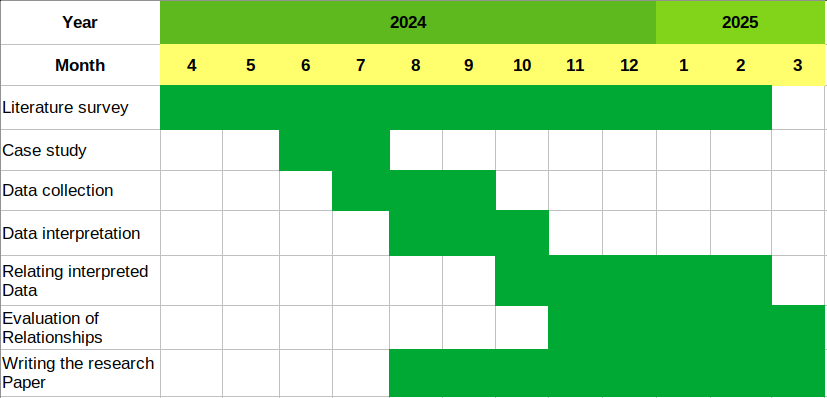
\includegraphics[width=0.65\textwidth]{timeline.png}
        \caption{Planned project timeline}
    \end{figure}

    \subsection{Current progress}
    \indent \par Currently literature survey and case study are going on, in parallel.

    \end{spacing}

    %List of References 
    \newpage
    \addcontentsline{toc}{section}{List of References }
    \section*{\begin{LARGE} List of References  \end{LARGE} }
    \printbibliography

\end{document}